
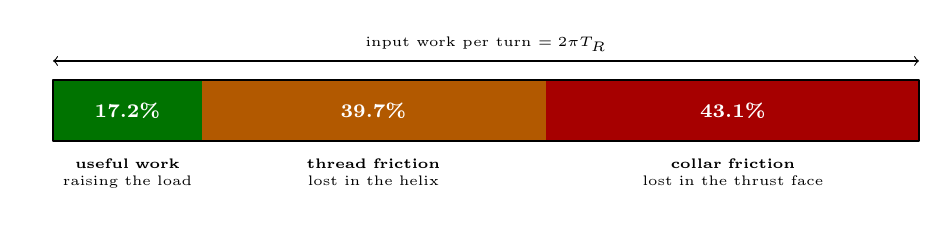
\begin{tikzpicture}[scale=1.0,font=\scriptsize,line join=round]
\def\W{11.0}
\fill[green!45!black] (0,0) rectangle (0.172*\W,0.78);
\fill[orange!70!black] (0.172*\W,0) rectangle (0.569*\W,0.78);
\fill[red!65!black] (0.569*\W,0) rectangle (\W,0.78);
\draw[thick] (0,0) rectangle (\W,0.78);
\node[white,font=\bfseries\scriptsize] at (0.086*\W,0.39) {17.2\%};
\node[white,font=\bfseries\scriptsize] at (0.370*\W,0.39) {39.7\%};
\node[white,font=\bfseries\scriptsize] at (0.785*\W,0.39) {43.1\%};
\node[anchor=north,align=center,font=\tiny,text width=2.3cm] at (0.086*\W,-0.10)
  {\textbf{useful work}\\ raising the load};
\node[anchor=north,align=center,font=\tiny,text width=3.0cm] at (0.370*\W,-0.10)
  {\textbf{thread friction}\\ lost in the helix};
\node[anchor=north,align=center,font=\tiny,text width=3.0cm] at (0.785*\W,-0.10)
  {\textbf{collar friction}\\ lost in the thrust face};
\draw[<->] (0,1.02) -- (\W,1.02) node[midway,above,font=\tiny]
  {input work per turn $=2\pi T_R$};
\end{tikzpicture}
